% !TeX TXS-program:compile = txs:///pdflatex/[--shell-escape]
% Le truc au-dessus pour avoir l'option shell-escape qui permet de faire du minted.
\documentclass[12pt]{article}

% Affichage ou non des reponses aux questions & exercices
\newif\ifDispRep
\DispReptrue  % Show the text
%\DispRepfalse % Hide the text

% Version du document
\newcommand{\versiondoc}{v0.1}

% Incorporation tous éléments de préambule communs à tous mes cours
% Sans chemin relatif parce que TexStudio lancé depuis un script qui prend en compte la variable d'environnement TEXINPUTS
\usepackage{CoursLFC}

% Eléments de l'en-tête et de la page de garde spécifiques à ce doc
\newcommand{\classe}{1\textsuperscript{ère} NSI}
\newcommand{\themecours}{Thème 6: Algorithmique}
\newcommand{\datedoc}{février 2024}

% Page de garde mise en page
\title
	{\vspace{3cm}
		{\Large
		\textit
			{
				\classe\hspace{0.1cm}
				\textemdash\
				\hspace{0.1cm}
				\themecours
			}
			
		\vspace{1cm}
		\huge{Algorithmique \& Mise au Point de Programmes} }
		 
		\vspace{1cm}
	}
\author{\etablissement}
\date{
	\auteur,
	\datedoc,
	\footnotesize{\textit{\versiondoc}} 
	\vspace{6cm}
	}

% Header & Footer
\lfoot{\etabshort}
\cfoot{\thepage}
\rfoot{\classe, \anneescol}
\renewcommand{\footrulewidth}{0.2pt}
\lhead{}
\chead{}
\rhead{}
\renewcommand{\headrulewidth}{0pt}

\begin{document}
	
	\maketitle
	% pas de footer sur la première page
	\thispagestyle{empty}
		
	\section*{}
		{\noindent
		\resumecours
		}
		
	\pagebreak	
	\tableofcontents
	
	\pagebreak
	
	% Début du contenu du document

	\section{Point d'étape -- où est-on / où va-t-on?}
	\subsection{Ce qu'on a couvert jusqu'à présent}
	
	\begin{itemize}
		\item Rudiments de l'architecture physique d'un ordinateur -- le modèle de Von Neumann.
		\item Mise en jambes sur de l'écriture de code: réalisation d'une page Web en HTML.
		\item Introduction à Python, et plus spécifiquement:
		\begin{itemize}
			\item Ce qu'on appelle ses "constructions élémentaires" -- variables, fonctions, conditions \& embranchements, boucles...
			\item Les types et valeurs de base: entiers (naturels et relatifs), flottants (réels), chaînes de caractères et booléens (qu'on n'a que brièvement abordés pour l'instant).
			\item Un type dit "construit" -- les listes.
		\end{itemize}
		\item Un peu de théorie: la représentation des types et valeurs de base en machine (les entiers naturels et relatifs, les réels, les alphanumériques).
		\item Un peu plus de théorie: introduction à la logique booléenne (que l'on n'a couverte que très rapidement -- on y reviendra en fin d'année).
		\item Un retour à la pratique: le traitement de données en table, la manipulation de fichiers dans Python, et des types de données plus complexes --- les dictionnaires, les listes de dictionnaires...
	\end{itemize}
	
	\subsection{Ce dont on va parler dans ce nouveau chapitre}
	On a donc fait des "sauts" de la théorie vers la pratique, puis vers la théorie de nouveau --- pour finalement atterrir ici, dans ce chapitre sur l'algorithmique qui se trouve presque exactement au "milieu" de cet axe théorie--pratique.
	
	Comme je vous l'ai dit à plusieurs reprises dans les parties précédentes -- et spécialement dans celle portant sur le traitement de données en table, l'algorithmique, vous en faites déjà: je vous pose des problèmes par le biais de notebooks Jupyter dans Capytale v2 et vous réfléchissez à comment les résoudre. Dit autrement, \textit{vous concevez des algorithmes}.
	
	Ce que l'on va faire dans ce nouveau chapitre c'est formaliser cette démarche, la structurer, puis étudier quelques exemples d'algorithmes beaucoup plus avancés que ce que l'on a vu jusqu'à présent.
	
	Spécifiquement, on va parcourir le chemin suivant:
	\begin{itemize}
		\item Introduction à l'algorithmique -- étapes de conception et de rédaction d'un algorithme;
		\item Pratique: tests d'algorithmes / de programmes;
		\item Preuve d'algorithmes;
		\item Complexité d'algorithmes;
		\item Etude de certains algorithmes spécifiques:
		\begin{itemize}
			\item Algorithme de recherche dichotomique dans un tableau;
			\item Algorithmes de tri - par sélection, par insertion;
			\item Algorithmes des k plus proches voisins -- algorithme d'apprentissage, "machine learning";
			\item Algorithmes gloutons.
		\end{itemize}
		\item Pratique: mise au point de programmes; programmation défensive.
	\end{itemize}
	
	\subsection{Comment on va procéder}
	Comme dit plus haut, on est ici à la frontière entre la théorie et la pratique -- on va donc avoir un fonctionnement hybride en classe:
	 \begin{itemize}
	 	\item \textbf{Prise de notes essentielle} --- vous commencez à connaître les cours que je vous fournis, il sont \textit{très} longs. Ils doivent vous servir de référence, vous permettre surtout de bien revoir les corrections d'exercices, mais votre savoir, lui, doit venir de votre prise de notes;
	 	\item Plusieurs exercices sur papier qu'on fera en classe et dont il sera très important que vous gardiez une trace;
	 	\item En parallèle et en complément, quelques applications / exercices sur machine.
	 \end{itemize}
	 
	 \pagebreak
	 
	 \section{Introduction à la conception d'algorithmes}
	 
	 Quelques questions pour commencer...
	 
	 \MaQuest{Qu'est-ce qu'un algorithme (indice: c'est constitué de trois parties)? }
	 \begin{MaReponse}
	 	Un algorithme est une \textbf{suite finie d'instructions} permettant de \textbf{résoudre un problème}. Il est structuré en trois parties:
		 \begin{alphenum}
		 	\item L'entrée des données;
		 	\item Le traitement des données;
		 	\item La sortie des données 
		 \end{alphenum}
	\end{MaReponse}
	
	\MaQuest{Parmi les éléments suivants, qu'est-ce qui est un algorithme, qu'est-ce qui n'en est pas?
		\begin{alphenum}
			\item Une recette de gâteau au chocolat;
			\item La liste des présidents de la V\textsuperscript{ème} République;
			\item Les règles du jeu d'échecs;
			\item Les règles à appliquer pour résoudre une équation du 2\textsuperscript{nd} degré;
			\item Les instructions de montage d'un meuble Ikea.
		\end{alphenum}
	}
	
	\begin{MaReponse}
		\begin{alphenum}
			\item Oui c'en est un -- ingrédients en entrée, étapes de confection, gâteau en sortie. C'est bien la résolution d'un problème (en l'occurrence "comment fabriquer un gâteau au chocolat?").
			\item Non ce n'en est pas un -- c'est une liste d'informations, pas des étapes à suivre.
			\item Ce n'en est pas un non plus -- ce n'est qu'une liste de principes. En revanche on pourrait les utiliser pour mettre en \oe{}uvre un algorithme qui joue aux échecs (et résoud le problème "comment jouer -- et gagner -- une partie d'échecs?).
			\item Oui c'en est un -- c'est même écrit dans la description ("résoudre").
			\item Oui c'en est un également.
		\end{alphenum}
	\end{MaReponse}
	
	\begin{MonAmp}{Définition}
		L'algorithmique est:
		\begin{itemize}
			\item La conception (et la production) d'algorithmes;
			\item Leur étude -- leur analyse, la mesure de leur fiabilité (est-ce qu'il répond vraiment au problème posé?) et de leur efficacité (est-ce qu'il le fait en un temps acceptable?).
		\end{itemize}
	\end{MonAmp}
	
	Nous allons dans ce cours nous intéresser à ces deux composantes, en commençant, dans ce chapitre, par la première dont les étapes peuvent se résumer ainsi:
	\begin{enumerate}
		\item Énoncé d'un problème à résoudre;
		\item Spécification de l'algorithme -- nom, entrées, sorties;
		\item Explicitation de la démarche en pseudo-code -- description du traitement des données qui va permettre de résoudre le problème;
		\item Traduction en langage de programmation.
	\end{enumerate}
	
	La 1\textsuperscript{ère} et la 4\textsuperscript{ème} étape sont à la marge de notre propos ici:
	\begin{itemize}
		\item L'énoncé d'un problème à résoudre par le biais d'un programme informatique est une activité à part entière (souvent appelée "expression de besoin" dans le monde professionnel). Vous y avez un petit peu touché dans le cadre de vos projets, mais dans l'ensemble, dans le contexte de la NSI, les problèmes vous sont posés -- et votre rôle consiste à savoir les résoudre;
		\item La traduction en langage de programmation, que dans le contexte de la NSI nous réalisons en Python, a fait l'objet d'un pan du cours distinct; nous allons évidemment y revenir en partie ici, mais la syntaxe Python n'est pas l'objet de notre étude ici.
	\end{itemize}
	
	\subsection{Écrire un algorithme: spécification}
	
	Avant d'écrire un algorithme il faut bien définir ce que l'on veut faire et à partir de quoi; il s'agit de donner \textbf{une spécification au problème}. Pour cela on doit:
	\begin{itemize}
		\item Donner un nom explicite à l’algorithme --- \textit{par exemple \texttt{CuissonGateauChocolat}};
		\item Décrire les conditions d'utilisation de l'algorithme, les données qu'il attend en entrée et les conditions dans lesquelles il va pouvoir être exécuté, sa \textbf{\textit{précondition}} --- \textit{par exemple "\texttt{Beurre et Lait non périmés}"}:
		\item De même, décrire le résultat attendu, sa \textbf{\textit{postcondition}}, la nature des données renvoyées et à quoi elles correspondent --- \textit{par exemple "\texttt{gâteau rond, moelleux, et succulent}"}.
	\end{itemize}
	
	Cette étape de spécification est fondamentale -- c'est en quelque sorte la "carte d'identité" de notre algorithme, ce qui va permettre à quelqu'un qui ne le connait pas de le comprendre sans avoir besoin de lire son code. On va donc la transcrire dans notre code Python en tête de la fonction lui correspondant -- et c'est exactement ce que je vous demande de faire dans vos projets.
	
	\begin{MonAmp}{Méthode}
		La transcription de la spécification d'un algorithme en tête de la fonction Python lui correspondant s'appelle "\textit{\textbf{le docstring}}" ou "\textit{\textbf{la documentation}}" de la fonction. Il est inscrit entre deux séries de trois apostrophes -- par exemple:
		\MonPython{001_Docstring.py}
	\end{MonAmp}
	
		\begin{MonExo}[Rédaction d'une spécification de fonction]
		Considérez la fonction suivante:
		\MonPython{002_MedianeNoDocstring.py}
		
		Est-ce que ce qu'elle fait est clair d'entrée de jeu? 
		
		Rédigez la docstring de cette fonction pour remédier à cela.
	\end{MonExo}
	
	\begin{MaReponse}
		On aura noté deux problèmes ici -- l'absence de docstring, mais également l'absence d'un nom explicite à la fonction ("Fonction", ce n'est franchement pas génial...). Remédions à tout cela:
		\MonPython{003_MedianeDocstring.py}
		Vous remarquerez l'inclusion d'exemples dans la docstring -- il ne faut surtout pas hésiter à y recourir, c'est ce qu'il y a de plus parlant pour quelqu'un qui découvre votre code!
	\end{MaReponse}
	
	\subsection{Ecrire un algorithme: pseudo-code}

	Si l'on se réfère aux étapes listées plus haut, on en est maintenant au moment où l'on sait \textit{ce que va réaliser} notre programme, \textit{ce qu'il va prendre en entrée}, et \textit{ce qu'il va retourner en sortie}. Il s'agit à présent d'expliciter le \textit{\textbf{comment}} -- quelles sont les étapes qui vont être effectuées pour résoudre le problème? Quel traitement va-t-on appliquer aux données en entrée pour produire les données en sortie?
	
	On a déjà utilisé à de multiples reprises le pseudo-code dans ce cours -- donc (\textit{en théorie}) vous devriez déjà être convaincus de son intérêt et savoir l'utiliser. Nous allons donc passer directement à quelques exercices d'application -- en rappelant tout de même au préalable les principes et règles suivants:
	\begin{alphenum}
		\item Le pseudo-code est une façon de décrire un algorithme pour qu'il soit compréhensible "entre humains".
		\item Le pseudo-code est indépendant du langage de programmation -- un algorithme convenablement écrit devrait en théorie pouvoir être implémenté aussi aisément en Python qu'en C ou qu'en JavaScript\footnote{C'est évidemment un peu simpliste d'écrire ceci ainsi, mais en théorie le principe est vrai: lorsque vous rédigez un algorithme en pseudo-code, vous devriez ne pas avoir de langage de programmation spécifique en tête.}. A titre d'exemple, voici un "Hello World" en deux langages de programmation distincts, mais partant du même pseudo-code:
		\begin{figure}[ht]
			\centering
			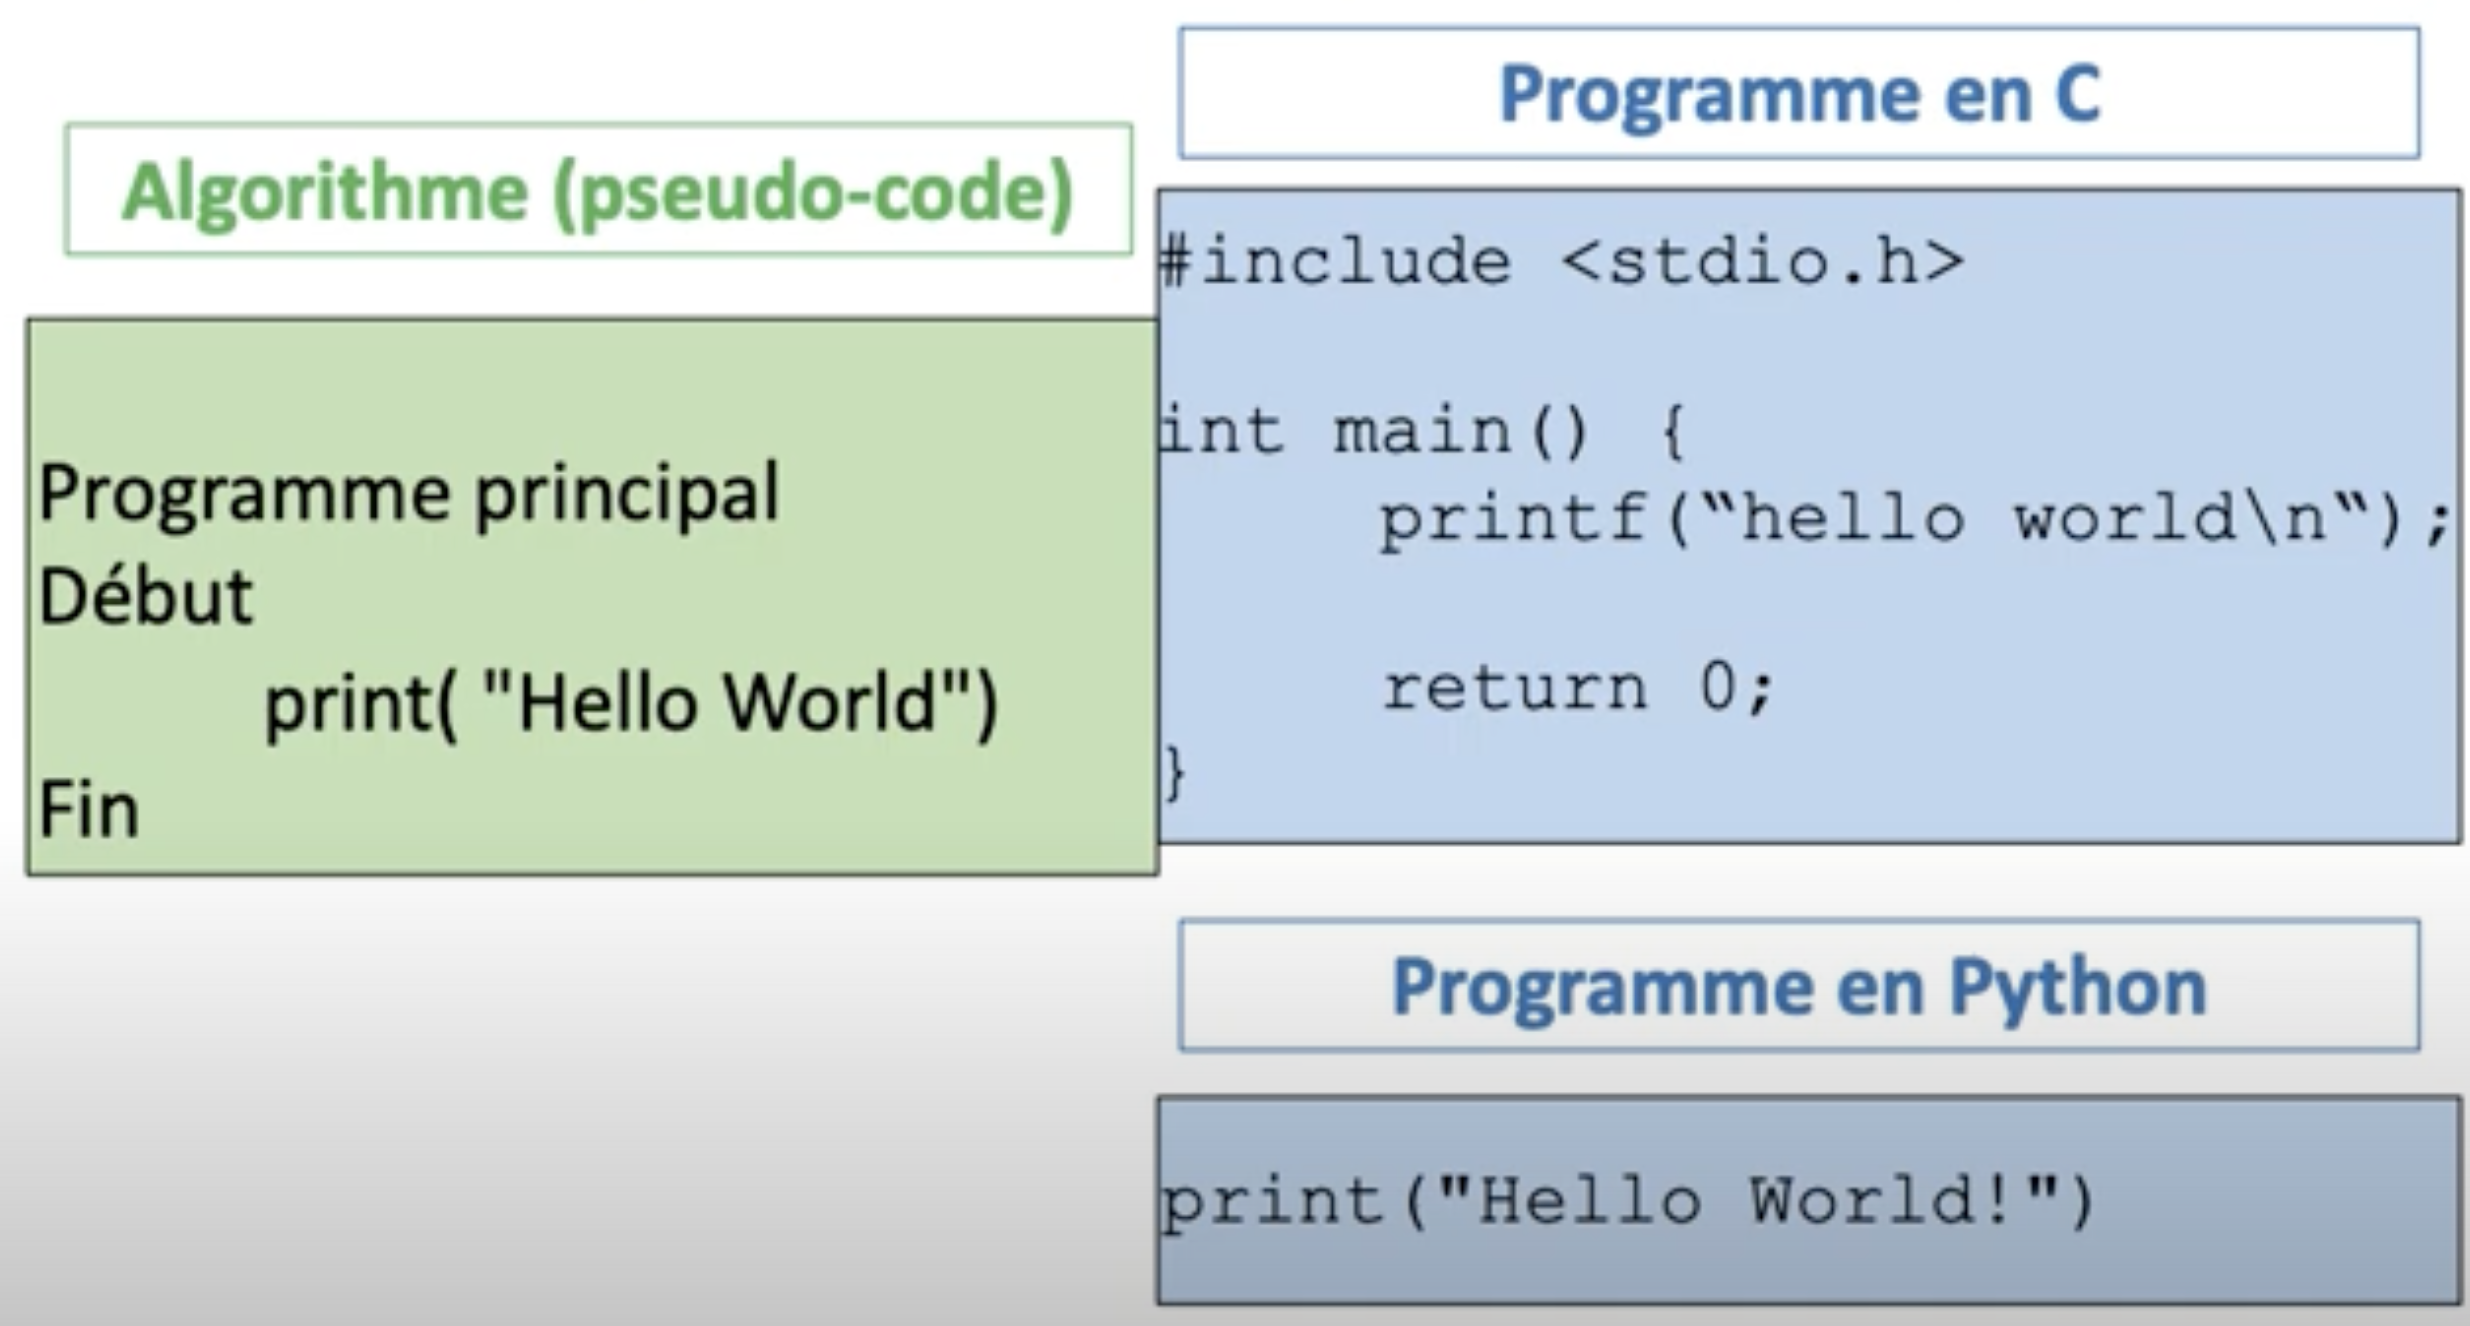
\includegraphics[width=0.5\textwidth]{001_AlgoHelloWorld.png}
		\end{figure}
		\item Conséquence: les règles de syntaxe de pseudo-code sont inspirées des éléments communs à la plupart des langages de programmation.
		\item Il n'y a pas de pseudo-code universel -- le seul principe à respecter, c'est que les règles de syntaxe appliquées soient bien définies, comprises et partagées par tous$\cdot$tes celles et ceux qui seront amené$\cdot$e$\cdot$s à lire les algorithmes.
	\end{alphenum}
	
	Ce dernier point implique qu'il y ait quand même une ossature de règles minimales dans un contexte donné -- comme pour ce cours par exemple:
	\begin{MonAmp}{Règles pseudo-code 1\textsuperscript{ère} NSI}
		\begin{alphenum}
			\item On spécifie explicitement en début d'algorithme les entrées attendues et les sorties prévues;
			\item On utilise une flèche vers la gauche ("$\leftarrow$" ou "$\lhd$") pour affecter des variables;
			\item On utilise l'indentation pour délimiter les fonctions, les conditions, les boucles...\footnote{Ici on triche un peu puisque l'indentation est spécifique à Python -- mais pas tant que ça puisque cela restera compréhensible même pour une implémentation dans un autre langage.}
			\item On explicite la fin de toute structure (fonction, condition, boucle...) débutée;
			\item On n'hésite pas à inclure des commentaires pour expliquer les étapes -- et dans ce cas, on les préfixe d'une flèche vers la droite ("$\rightarrow$" ou "$\rhd$")
			\item ... et c'est tout!
		\end{alphenum}
	\end{MonAmp}	 
	
	Pour illustrer ces principes, voici le pseudo-code d'une fonction (qu'on a déjà vue dans un chapitre précédent, d'ailleurs) prenant une liste de réels positifs en entrée et qui en renvoie le maximum:
	
	\vspace{\baselineskip}
	
	\begin{algorithmic}[1]
		\Require{$liste$ dont tous les éléments $\in \mathds{R+}$}
		\Ensure{$Max \in \mathds{R+}$}
		\Function{TrouveMax}{liste}
		\State Max $\leftarrow$ 0
		\ForAll{$Element$ de liste}
		\If{$Element > Max$}
		\Comment{On a trouvé un nouveau max}
		\State $Max$ $\leftarrow Element$
		\EndIf
		\EndFor
		\State\Return{$Max$}
		\EndFunction
	\end{algorithmic}
	
		\begin{MonExo}[Rédaction d'algorithmes en pseudo-code]
		En appliquant les principes énoncés ci-dessus, rédigez les algorithmes suivants:
		\begin{alphenum}
			\item Un algorithme qui prend deux nombres en entrée et affiche leur somme.
			\item Un algorithme qui calcule la somme des N premiers entiers naturels.
			\item Un algorithme qui génère les N premiers termes de la séquence de Fibonacci. (rappel: c'est une suite de nombres dont les deux premiers sont 0 et 1 et dont chaque élément est la somme des deux précédents -- donc: 0, 1, 1, 2, 3, 5, 8, 13, etc...).
			\item Un algorithme qui vérifie si une chaîne de caractères est un palindrome (se lit de la même manière dans les deux sens).
			\item \textbf{$[$BONUS$]$} --- Supposez que vous avez une liste Lst de nombres réels  ordonnée (c'est-à-dire où $Lst[0] \leq Lst[1] \leq (...) \leq Lst[n]$) et que vous cherchez à savoir si elle contient un nombre N en particulier (la conclusion sera donc booléenne - Vrai ou Faux). Rédigez puis comparez deux algorithmes:
			\begin{itemize}
				\item Un qui fait une recherche "normale", en commençant à un bout et en parcourant toute la liste;
				\item Un  autre qui effectue une recherche dite "dichotomique":
				\begin{itemize}
					\item Il regarde le milieu de la liste: 
					\begin{itemize}
						\item S'il est supérieur à N il élimine la partie supérieure de la liste;
						\item S'il est inférieur à N il élimine la partie inférieure de la liste;
					\end{itemize}
					\item Il recommence l'opération jusqu'à soit trouver N soit aboutir à une impossibilité.
				\end{itemize}
			\end{itemize}
			Que peut-on dire des efficacités relatives de ces deux algorithmes?
		\end{alphenum}
	\end{MonExo}
	
	\begin{MaReponse}
		Il n'y a jamais (ou rarement) une solution algorithmique unique à un problème -- ce qui suit n'est donc que des propositions de solution (qui sont, évidemment, valides -- mais pas uniques).
		\begin{alphenum}
			\item
			\begin{algorithmic}[1]
				\Require{deux nombres $a$ et $b$ $\in \mathds{R}$}
				\Ensure{$a + b$}
				\Function{Somme}{a, b}
				\State Resultat $\leftarrow$ a + b
				\State\Return{$Resultat$}
				\EndFunction
			\end{algorithmic}
			\vspace{\baselineskip}
			\item
			\begin{algorithmic}[1]
				\Require{$N$ $\in \mathds{N}$}
				\Ensure{la somme des N premiers entiers naturels}
				\Function{SommeEntiers}{N}
				\State $Resultat$ $\leftarrow$ 0
				\Comment{On  initialise le résultat à 0}
				\For{$i$ allant de 1 à N}
				\State $Resultat$ $\leftarrow Resultat + i$
				\EndFor
				\State\Return{$Resultat$}
				\EndFunction
			\end{algorithmic}
			\vspace{\baselineskip}
			\item
			\begin{algorithmic}[1]
				\Require{$N$ $\in \mathds{N}$ avec $N \geq 2$}
				\Comment{On précise bien les valeurs acceptables en entrée}
				\Ensure{aucune}
				\Comment{On va afficher les résultats, pas les retourner}
				\Function{Fibonacci}{N}
				\State ValeurPrec $\leftarrow$ 0
				\State ValeurCour $\leftarrow$ 1
				\State Afficher ValeurPrec
				\Comment{On affiche le 0 puis on rentre dans la boucle}
				\For{$i$ allant de 2 à N}
				\State Afficher ValeurCour
				\State Suivant $\leftarrow$ $ValeurPrec + ValeurCour$
				\State ValeurPrec $\leftarrow$ ValeurCour
				\State ValeurCour $\leftarrow$ Suivant
				\EndFor
				\EndFunction
			\end{algorithmic}
			\vspace{\baselineskip}
			\item
			\begin{algorithmic}[1]
				\Require{chn, une chaine de caractères}
				\Ensure{$Vrai$ ou $Faux$ selon si la chaine est un palindrome ou non}
				\Function{EstPalindrome}{chn}
				\State $Long$ $\leftarrow$ $longueur(chn)$
				\If{$Long$ est pair}
				\State $Milieu$ $\leftarrow$ $Long / 2$
				\Else
				\State $Milieu$ $\leftarrow$ $(Long  - 1) / 2$
				\EndIf
				\For{$i$ allant de 0 à Milieu}
				\If{$chn[i] \neq chn[Long - i]$}
				\State\Return{$Faux$}
				\EndIf
				\EndFor
				\State\Return{$Vrai$}
				\EndFunction
			\end{algorithmic}
			Quelques remarques sur cet algorithme:
			\begin{itemize}
				\item Lignes 8 et 9: le but ici est de bien comprendre l'algorithme -- avec cette formule on comprend bien ce qu'on fait: on part du début pour aller jusqu'au milieu. Strictement parlant les formules ne marchent pas (en Python chn[Long] donnerait une erreur) -- mais on s'en fiche: la démarche est claire ici, et c'est le but.
				\item Ligne 3: on vérifie la parité de la longueur puisque dans le cas des longueurs impaires on ignorera le caractère du milieu. Vous noterez qu'on dit ici "si Long est pair" sans expliquer comment on fait -- la difficulté de l'algorithme n'étant pas là, c'est tout à fait acceptable (on imagine qu'il y aura un algorithme pour une fonction "EstPair" explicité ailleurs).
				\item Lignes 10 et 13: c'est une démarche qu'on a déjà utilisée ailleurs pendant notre cours, qui est très classique, et qu'il faut impérativement maîtriser: on part du principe que quelque chose est vrai --- ici "chaîne est un palindrome" --- et dès qu'on trouve une preuve du contraire (ici: un caractère est différent de son homologue de l'autre côté) on retourne "Faux", c'est-à-dire qu'on arrête immédiatement la fonction puisqu'on connaît son résultat. Si on arrive au bout de la boucle, c'est qu'on a pas trouvé de preuve que c'est faux -- donc c'est vrai et c'est ce qu'on retourne.
			\end{itemize}
		\end{alphenum}
	\end{MaReponse}
	
	\begin{MonExo}[Traduction de pseudo-code en Python]
		\begin{alphenum}
			\item Choisissez l'un des des deux derniers algorithmes de la question précédente (éléments de la suite de Fibonacci ou vérification de palindrome) et traduisez-le en une fonction Python.
			\item \textbf{Expliquez comment vous allez tester votre fonction.}
			\item \textbf{$[$BONUS$]$} --- Traduisez en Python l'algorithme de recherche dichotomique.
		\end{alphenum}
	\end{MonExo}
	
	\begin{MaReponse}
		Pour la suite de Fibonacci, on pourra utiliser le code suivant:
		\MonPython{004_Fibonacci.py}
		Pour la tester, il suffira de la lancer avec différentes valeurs de N et de vérifier que le résultat est correct. Assez rapidement on constatera que si l'on passe une valeur de N qui n'est pas dans le champ des possibles (1, par exemple, ou -2) alors on rencontre une erreur -- nous reviendrons plus tard dans ce cours sur comment gérer cela.
		
		\vspace{\baselineskip}
		Pour le palindrome, on pourra utiliser le code suivant:
		\MonPython{005_Palindrome.py}
		Pour la tester, il faudra réfléchir un peu plus à tous les cas de figures possibles:
		\begin{itemize}
			\item Chaine de longueur paire qui est un palindrome;
			\item Chaine de longueur paire qui n'en est pas un;
			\item Chaine de longueur impaire qui est un palindrome;
			\item Chaine de longueur impaire qui n'en est pas un.
		\end{itemize}
	\end{MaReponse}
	
		 \subsection{Tester un algorithme}
	
	Cette étape est cruciale dans le développement d'un programme informatique car les erreurs dans les phases de rédaction de l'algorithme et de traduction en langage de programmation sont plus que fréquentes -- elles sont systématiques dès lors qu'un programme atteint un certain niveau de complexité.
	
	\pagebreak
	\section{Preuve et complexité d'algorithmes}

\end{document}


%Eléments manquants:
%Section pseudo-code:
%- Le pseudo code des deux tris et la discussion de la comparaison dans l'exercice 2
%- Le code de la recherche dichotomique dans l'exercice 3
